\section{Polynomien kertolasku}

\qrlinkki{http://opetus.tv/maa/maa2/polynomien-kertolasku/}
{Opetus.tv: \emph{polynomien kertolasku} (10:00)}

Polynomilausekkeiden käsittely on välttämätön taito matematiikassa, ja siksi tähän lukuun kannattaa paneutua kunnolla.

\subsubsection*{Monomien tulo}

Kahden monomin tulo sievennetään kertomalla kertoimet keskenään ja kirjainosat keskenään. Muista potenssien laskusäännöt!

\begin{esimerkki}
Laske \quad a) $2x\cdot 3x$ \quad b)$-3x^2\cdot (-5x^4)$ \quad 
c) $5x^2 \cdot (-2x)$
\begin{esimratk}
\begin{enumerate}[a)]
    \item $2x\cdot 3x = 2\cdot 3\cdot x\cdot x = 6x^2$
    \item $-3x^2\cdot (-5x^4) = (-3)\cdot (-5) \cdot x^2 \cdot x^4 = 15 x^6$
    \item $5x^2 \cdot (-2x) = -10 x^3$
\end{enumerate}
\end{esimratk}
\begin{esimvast}
a) $6x^2$ \quad b) $15x^6$ \quad c) $-10x^3$
\end{esimvast}
\end{esimerkki}

\subsubsection*{Polynomin kertominen monomilla}

Polynomeja voi kertoa keskenään reaalilukujen tuttujen laskusääntöjen avulla. Yksinkertaisin erikoistapaus on polynomin kertominen monomilla, jolloin
käytetään osittelulakia $a(b+c)=ab+ac$.

\begin{esimerkki}
Laske \quad a) $5(x+3)$ \quad b) $2x(x-5)$ \quad 
c) $3(a+b+c)$
\begin{enumerate}[a)]
    \item $5(x+3) = 5\cdot x + 5\cdot 3 = 5x+15$
    \item $2x(x-5)=2x^2-10x$
    \item $3(a+b+c)=3a+3b+3c$
\end{enumerate}
\end{esimerkki} 

\subsubsection*{Kahden binomin tulo}

Kahden binomin tulossa kummallakin ensimmäisen binomin termillä kerrotaan toisen binomin termit. Saadut neljä tuloa lasketaan yhteen. 

\newcommand{\pbezier}[4]{
	\pgfmathsetmacro{\PBxa}{#1}
	\pgfmathsetmacro{\PBxb}{#2}
	\pgfmathsetmacro{\PBya}{#3}
	\pgfmathsetmacro{\PByb}{#3+#4}
	\pgfmathsetmacro{\PBca}{0.8 * \PBxa + 0.2 * \PBxb}
	\pgfmathsetmacro{\PBcb}{0.2 * \PBxa + 0.8 * \PBxb}
	\draw[color=red] (\PBxa, \PBya) .. controls (\PBca, \PByb) and (\PBcb, \PByb) .. (\PBxb, \PBya);
}

\begin{esimerkki}
Laske binomien $x+2$ ja $x-5$ tulo. \\
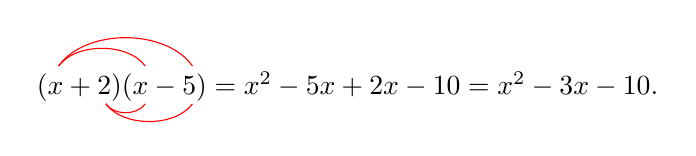
\begin{tikzpicture}
\draw node[right] {$(x+2)(x-5) = x^2-5x+2x-10 = x^2 -3x-10.$};

\pgfmathsetmacro{\klAx}{0.40}
\pgfmathsetmacro{\klBx}{1.00}
\pgfmathsetmacro{\klCx}{1.5}
\pgfmathsetmacro{\klDx}{2.1} % oli 2.8
\pgfmathsetmacro{\klEx}{3.64}
\pgfmathsetmacro{\klLo}{-0.22}
\pgfmathsetmacro{\klHi}{0.26}

\pbezier{\klAx}{\klCx}{\klHi}{0.3}
\pbezier{\klAx}{\klDx}{\klHi}{0.48}

\pbezier{\klBx}{\klCx}{\klLo}{-0.15}
\pbezier{\klBx}{\klDx}{\klLo}{-0.3}
\end{tikzpicture}\newline
\end{esimerkki}

\begin{esimerkki}
Laske binomien $x^2-x$ ja $2x-1$ tulo. \\
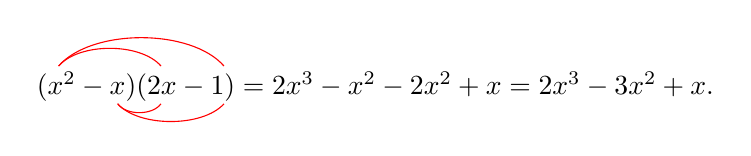
\begin{tikzpicture}
\draw node[right] {$(x^2-x)(2x-1) = 2x^3-x^2-2x^2+x = 2x^3 -3x^2 +x.$};

\pgfmathsetmacro{\klAx}{0.40}
\pgfmathsetmacro{\klBx}{1.15}
\pgfmathsetmacro{\klCx}{1.7}
\pgfmathsetmacro{\klDx}{2.5}
\pgfmathsetmacro{\klEx}{3.64}
\pgfmathsetmacro{\klLo}{-0.22}
\pgfmathsetmacro{\klHi}{0.26}

\pbezier{\klAx}{\klCx}{\klHi}{0.3}
\pbezier{\klAx}{\klDx}{\klHi}{0.48}

\pbezier{\klBx}{\klCx}{\klLo}{-0.15}
\pbezier{\klBx}{\klDx}{\klLo}{-0.3}
\end{tikzpicture}\newline
\end{esimerkki}

\subsubsection*{Yleinen kertolasku}

Osittelulain nojalla kahden polynomin tulo saadaan laskemalla yhteen kaikki
termit, jotka saadaan kertomalla termi ensimmäisestä ja toinen termi toisesta
polynomista.


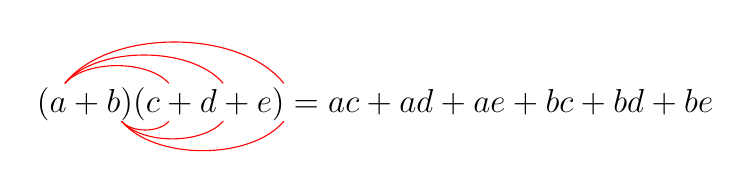
\begin{tikzpicture}
\draw node[right] {\large $(a+b)(c+d+e) = ac+ad+ae+bc+bd+be$};

\pgfmathsetmacro{\klAx}{0.48}
\pgfmathsetmacro{\klBx}{1.20}
\pgfmathsetmacro{\klCx}{1.8}
\pgfmathsetmacro{\klDx}{2.49}
\pgfmathsetmacro{\klEx}{3.26}
\pgfmathsetmacro{\klLo}{-0.22}
\pgfmathsetmacro{\klHi}{0.26}

\pbezier{\klAx}{\klCx}{\klHi}{0.3}
\pbezier{\klAx}{\klDx}{\klHi}{0.48}
\pbezier{\klAx}{\klEx}{\klHi}{0.7}

\pbezier{\klBx}{\klCx}{\klLo}{-0.15}
\pbezier{\klBx}{\klDx}{\klLo}{-0.3}
\pbezier{\klBx}{\klEx}{\klLo}{-0.5}
\end{tikzpicture}

\begin{esimerkki}
Laske polynomien $x-3$ ja $x^2-4x+3$ tulo. \\
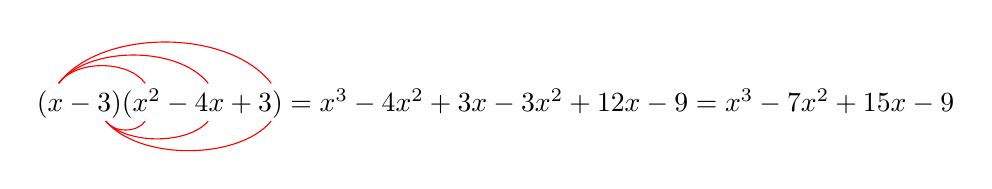
\begin{tikzpicture}
\draw node[right] {$(x-3)(x^2-4x+3) = x^3-4x^2+3x-3x^2+12x-9 = x^3-7x^2+15x-9$};

\pgfmathsetmacro{\klAx}{0.40}
\pgfmathsetmacro{\klBx}{1.00}
\pgfmathsetmacro{\klCx}{1.5}
\pgfmathsetmacro{\klDx}{2.3}
\pgfmathsetmacro{\klEx}{3.1}
\pgfmathsetmacro{\klLo}{-0.22}
\pgfmathsetmacro{\klHi}{0.26}

\pbezier{\klAx}{\klCx}{\klHi}{0.3}
\pbezier{\klAx}{\klDx}{\klHi}{0.48}
\pbezier{\klAx}{\klEx}{\klHi}{0.7}

\pbezier{\klBx}{\klCx}{\klLo}{-0.15}
\pbezier{\klBx}{\klDx}{\klLo}{-0.3}
\pbezier{\klBx}{\klEx}{\klLo}{-0.5}
\end{tikzpicture}\newline
\end{esimerkki}

\begin{esimerkki}
Laske polynomien $x^4-3x^3+3$ ja $x^3-2x^2+1$ tulo. \\
\begin{align*}
&\hspace{0.5cm}(\textcolor{red}{x^4} \textcolor{blue}{-3x^3} +{}\textcolor{green}{3})(x^3-2x^2+1) \\
&= \textcolor{red}{x^4}\cdot x^3 + \textcolor{red}{x^4}\cdot (-2x^2)+\textcolor{red}{x^4}\cdot 1\textcolor{blue}{{}-3x^3}\cdot x^3\textcolor{blue}{{}-3x^3}\cdot(-2x^2)\textcolor{blue}{{}-3x^3}\cdot1 \\
&\hspace{0.5cm}+\textcolor{green}{3}x^3+\textcolor{green}{3}\cdot(-2x^2)+\textcolor{green}{3}\cdot 1 \\
&= x^7-2x^6+x^4-3x^6+6x^5-3x^3+3x^3-6x^2+3 \\
&= x^7-5x^6+6x^5+x^4-6x^2+3
\end{align*}
\end{esimerkki}

\subsection*{Muistikaavat}

\qrlinkki{http://opetus.tv/maa/maa2/muistikaavat/}{
Opetus.tv: \emph{muistikaavat} (8:05, 6:38 ja 9:08)}

Joitakin polynomien kertolaskuja tarvitaan niin usein, että niitä kutsutaan \termi{muistikaavat}{muistikaavoiksi}.

\laatikko{
    \textbf{Muistikaavat}
    \begin{itemize}
        \item $(a+b)^2 = a^2+2ab+b^2$
        \item $(a-b)^2 = a^2-2ab+b^2$
        \item $(a+b)(a-b) = a^2-b^2$
    \end{itemize}
}

Nämä kaavat voidaan todistaa helposti laskemalla.

\paragraph*{Summan neliö}

\begin{align*}
(a+b)^2 &= (a+b)(a+b) &\emph{neliön määritelmä} \\
% &= a(a+b)+b(a+b) &\emph{osittelulaki} \\
&= a^2+ab+ba+b^2 &\emph{osittelulaki} \\
&= a^2+ab+ab+b^2 &\emph{vaihdannaisuus ($ba=ab$)} \\
&= a^2+2ab+b^2
\end{align*}

\paragraph*{Erotuksen neliö}

\begin{align*}
(a-b)^2 &= (a-b)(a-b) &\emph{neliön määritelmä} \\
% &= a(a-b)-b(a-b) &\emph{osittelulaki} \\
&= a^2-ab-ba+b^2 &\emph{osittelulaki} \\
&= a^2-ab-ab+b^2 &\emph{vaihdannaisuus ($ba=ab$)} \\
&= a^2-2ab+b^2
\end{align*}

Edellä todistettuja kahta muistikaavaa kutsutaan yhdessä nimellä binomin neliö. Toisinaan ne kirjoitetaan yhtenä yhtälönä muodossa $(a \pm b)^2=a^2 \pm 2ab+b^2$. % Kaavoissa useasti esiintyviä $\pm$-merkkejä luetaan siten, että ylemmät ja alemmat täsmäävät keskenään. Ylempien merkkien (kaikki $+$:ia) valinta vastaa siis summan neliötä ja alempien merkkien (kaikki $-$:ia) valinta erotuksen neliötä.

\paragraph*{Summan ja erotuksen tulo}

\begin{align*}
(a+b)(a-b) &= a^2-ab+ba-b^2 &\emph{osittelulaki} \\
&= a^2-ab+ab-b^2 &\emph{vaihdannaisuus ($ba=ab$)} \\
&= a^2-b^2
\end{align*}

\begin{esimerkki}
Sievennä $(3x-2y)^2$. \\
\quad\\
Käytetään muistikaavaa $(a-b)^2 = a^2-2ab+b^2$. Nyt $a = 3x$ ja $b = 2y$.
Saadaan
        \[ (3x+2y)^2 = (3x)^2-2\cdot 3x\cdot 2y+(2y)^2 = 9x^2-12xy+4y^2. \]
\end{esimerkki}

\begin{esimerkki}
Laske ilman laskinta a) $995^2$ b) $104 \cdot 96$. \\
Käytetään ovelasti muistikaavoja $(a-b)^2 = a^2-2ab+b^2$ ja \mbox{$(a+b)(a-b) = a^2-b^2$}.
\begin{enumerate}[a)]
\item $995^2 = (1000-5)^2 = 1000^2-2\cdot 1000\cdot 5+5^2 = 1000000-10000+25 = 990025 $
\item $104\cdot 96 = (100+4)(100-4) = 100^2 - 4^2 = 10000 - 16 = 9984$.
\end{enumerate}
\end{esimerkki}

\begin{tehtavasivu}

\paragraph*{Opi perusteet}

\begin{tehtava}
    Sievennä.
    \begin{enumerate}[a)]
        \item $2(x+3)$
        \item $x(x - 2)$
        \item $3x(1-2x)$
        \item $x^2(x + 5)$
    \end{enumerate}
    \begin{vastaus}
        \begin{enumerate}[a)]
            \item $2x+6$
            \item $x^2 - 2x$
            \item $3x-6x^2$
            \item $x^3 + 5x$
        \end{enumerate}
    \end{vastaus}
\end{tehtava}

\begin{tehtava}
    Sievennä.
    \begin{enumerate}[a)]
        \item $3(x+2y-4)$
        \item $(x+2)(x + 3)$
        \item $(3-x)(2x-1)$
\end{enumerate}
    \begin{vastaus}
        \begin{enumerate}[a)]
            \item $3x+6y-12$
            \item $x^2 +5x+6$
            \item $-2x^2+7x-3$
        \end{enumerate}
    \end{vastaus}
\end{tehtava}

\begin{tehtava}
    Kerro sulut auki muistikaavan avulla.
    \begin{enumerate}[a)]
        \item $(x+y)^2$
        \item $(x-y)^2$
        \item $(x+y)(x-y)$
    \end{enumerate}
    \begin{vastaus}
        \begin{enumerate}[a)]
        \item $x^2 +2xy+y^2$
        \item $x^2 -2xy +y^2$
        \item $x^2-y^2$
        \end{enumerate}
    \end{vastaus}
\end{tehtava}

\begin{tehtava}
    Kerro sulut auki muistikaavan avulla.
    \begin{enumerate}[a)]
        \item $(x+3)^2$
        \item $(y-5)^2$
        \item $(x-4)(x+4)$
        \item $(3x+2)^2$
    \end{enumerate}
    \begin{vastaus}
        \begin{enumerate}[a)]
        \item $x^2 +6x+9$
        \item $y^2 - 10y+25$
        \item $x^2 -16$
        \item $9x^2 +12x +4$
        \end{enumerate}
    \end{vastaus}
\end{tehtava}

\begin{tehtava}
    Sievennä lauseke $(x^2+1)(x^3-2x)$. Mikä on polynomin aste?
    \begin{vastaus}
        Lauseke sievenee muotoon $x^5-x^3-2x$. Polynomin aste on $5$.
    \end{vastaus}
\end{tehtava}

\paragraph*{Hallitse kokonaisuus}

\begin{tehtava}
    Pohdi ja määritä sulkuja avaamatta lausekkeen $(x^2+1)(x^3-2x)$
    \begin{enumerate}[a)]
        \item aste
        \item vakiotermi.
    \end{enumerate}
    \begin{vastaus}
        \begin{enumerate}[a)]
            \item Polynomin aste on kunkin tekijän korkeimpien asteiden summa, tässä siis $2+3=5$.
            \item Polynomin vakiotermi on kunkin tekijän vakiotermien tulo, tässä siis $1\cdot 0=0$.
        \end{enumerate}
    \end{vastaus}
\end{tehtava}

\begin{tehtava}
    Sievennä.
    \begin{enumerate}[a)]
        \item $(-2x)(4x - 1)\cdot 3$
        \item $(-x^3)(10x - 2)$
        \item $5(-2x + 1)(-9x) $
        \item $2x(x-3)+1$
    \end{enumerate}
    \begin{vastaus}
        \begin{enumerate}[a)]
            \item $-24x^2 + 6x$
            \item $-10x^4 + 2x^3$
            \item $90x^2 - 45x$
            \item $2x^2-6x+1$
        \end{enumerate}
    \end{vastaus}
\end{tehtava}

\begin{tehtava}
    Sievennä muistikaavojen avulla.
    \begin{enumerate}[a)]
        \item $(5-x)^2$
        \item $(7x + 4)^2$
        \item $(9 - 7x)(9 + 7x)$
        \item $(8x - 8)(8x + 8)$
    \end{enumerate}
    \begin{vastaus}
        \begin{enumerate}[a)]
            \item $x^2 - 10x + 25$
            \item $49x^2 + 56x + 16$
            \item $-49x^2 + 81$
            \item $64x^2 - 64$
        \end{enumerate}
    \end{vastaus}
\end{tehtava}

\begin{tehtava}
    Sievennä.
    \begin{enumerate}[a)]
        \item $(2y+5)(y+7)$
        \item $(x-1)(x+4)x$
    \end{enumerate}
    \begin{vastaus}
        \begin{enumerate}[a)]
            \item $2y^2 + 19y + 35$
            \item $x^3 + 3x^2 - 4x$
        \end{enumerate}
    \end{vastaus}
\end{tehtava}

\begin{tehtava}
    Sievennä.
    \begin{enumerate}[a)]
        \item $(t+v)^2+(t-v)^2$
        \item $(t+v)^2-(t-v)^2$
    \end{enumerate}
    \begin{vastaus}
        \begin{enumerate}[a)]
            \item $(t+v)^2+(t-v)^2 = t^2+2tv+v^2+t^2-2tv+v^2 = 2t^2+2v^2$
            \item $(t+v)^2-(t-v)^2 = t^2+2tv+v^2-t^2+2tv-v^2 = 4tv$
        \end{enumerate}
    \end{vastaus}
\end{tehtava}

\paragraph*{Lisää tehtäviä}

\begin{tehtava}
	Sievennä. 
	\begin{enumerate}[a)]
		\item $(x-3)(2x^3-3x+4)$
		\item $(x^2+1)(x^3-2x-4)$
		\item $(x-1)(x^4+x^3+x^2+x+1)$
		\item $(\frac x5-\frac23)(x^2+x+1)$
	\end{enumerate}
	\begin{vastaus}
		\begin{enumerate}[a)]
			\item $2x^4-6x^3-3x^2+13x-12$
			\item $x^5-x^3-4x^2-2x-4$
			\item $x^5-1$
			\item $\frac15x^3-\frac{7}{15}x^2-\frac{7}{15}x-\frac23$
		\end{enumerate}
	\end{vastaus}
\end{tehtava}

\begin{tehtava}
    Sievennä.
    \begin{enumerate}[a)]
            \item $(a+b)^3$
            \item $(a+b)^4$
            \item $(a-b)^3$
        \end{enumerate}
    \begin{vastaus}
        \begin{enumerate}[a)]
            \item $(a+b)^3 = a^3 + 3a^2b + 3ab^2 + b^3$
            \item $(a+b)^4 = a^4 + 4a^3b + 6a^2b^2 + 4ab^3 + b^4$
            \item $(a-b)^3 = a^3 - 3a^2b + 3ab^2 - b^3$
        \end{enumerate}
    \end{vastaus}
\end{tehtava}

\begin{tehtava}
    Sievennä. (Ohje: käytä summakaavoja.)
    \begin{enumerate}[a)]
        \item $63^2+37^2$
        \item $101^2+99^2$
    \end{enumerate}
    \begin{vastaus}
        \begin{enumerate}[a)]
            \item $63^2+37^2 = (50+13)^2+(50-13)^2 = 2\cdot 50^2 + 2\cdot 13^2 = 2\cdot 2500 +2\cdot 169 = 5000 + 338 = 5338$
            \item $101^2+99^2 = (100+1)^2+(100-1)^2 = 2\cdot 100^2 + 2\cdot 1^2 = 2\cdot 10000 + 2\cdot 1 = 20000 + 2 = 20002$
        \end{enumerate}
    \end{vastaus}
\end{tehtava}

\begin{tehtava}
    Sievennä.
    \begin{enumerate}[a)]
        \item $35^2-25^2$
        \item $170^2-50^2$
    \end{enumerate}
    \begin{vastaus}
        \begin{enumerate}[a)]
            \item $35^2-25^2 = (30+5)^2-(30-5)^2 = 4\cdot 30\cdot 5 = 600$
            \item $170^2-30^2 = (100+70)^2+(100-70)^2 = 4\cdot 100\cdot 70 = 28000$
        \end{enumerate}
    \end{vastaus}
\end{tehtava}

\begin{tehtava} %Vaikea!
    $\star$ Kahden luvun keskiarvo on $7$. Kuinka suuri niiden tulo voi korkeintaan olla?
    \begin{vastaus}
        $49$. Perustelu muistikaavoilla: $(7+a)(7-a)=7^2-a^2 = 49-a^2 \geq 49$
    \end{vastaus}
\end{tehtava}

\begin{tehtava}
    Olkoon $P(x)=-x^4+2x$ reaalifunktio. Sievennä lausekkeet.
    \begin{enumerate}[a)]
		\item $P(\sqrt{2})$
        \item $P(x)^2$
        \item $P(-x)$
        \item $P(2t)$
    \end{enumerate}
    \begin{vastaus}
        \begin{enumerate}[a)]
            \item $-4 + 2\sqrt{2}$
            \item $x^8 - 4x^5 + 4x^2$
            \item $-x^4-2x$
            \item $-16t^4+4t$
        \end{enumerate}
    \end{vastaus}
\end{tehtava}

\begin{tehtava}
    Olkoot $P(x)=x^2$ ja $Q(x)=x+1$ reaalifunktioita. Sievennä lausekkeet.
    \begin{enumerate}[a)]
        \item $P(x+1)$
        \item $Q(x-1)$
        \item $P(Q(x))$
        \item $Q(P(x))$
    \end{enumerate}
    \begin{vastaus}
        \begin{enumerate}[a)]
            \item $P(x+1) = (x+1)^2 = x^2+2x+1$
            \item $Q(x-1) = (x-1)+1 = x$
            \item $P(Q(x)) = P(x+1) = (x+1)^2 = x^2+2x+1$
            \item $Q(P(x)) = Q(x^2) = x^2+1$
        \end{enumerate}
    \end{vastaus}
\end{tehtava}

\end{tehtavasivu}
